\begin{figure}[htbp]
\centering
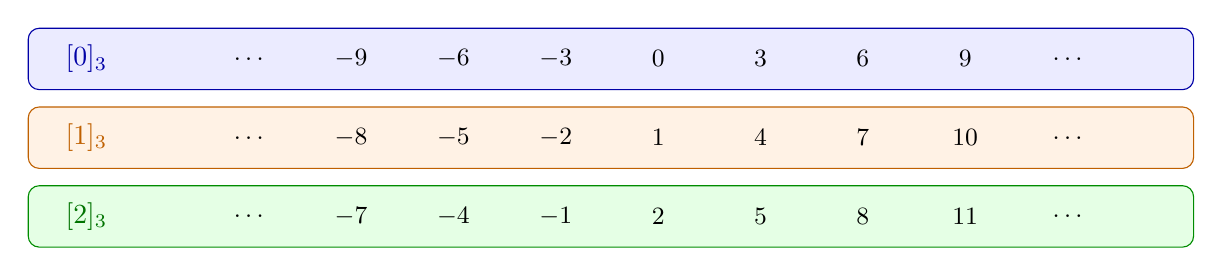
\begin{tikzpicture}[font=\small]
    \node[draw=blue!65!black,fill=blue!8,rounded corners,minimum width=14.8cm,minimum height=0.78cm,inner sep=2pt] at (7.4,2) {};
    \node[draw=orange!75!black,fill=orange!10,rounded corners,minimum width=14.8cm,minimum height=0.78cm,inner sep=2pt] at (7.4,1) {};
    \node[draw=green!55!black,fill=green!10,rounded corners,minimum width=14.8cm,minimum height=0.78cm,inner sep=2pt] at (7.4,0) {};
    \node[anchor=west,text=blue!65!black,font=\bfseries] at (0.35,2) {$[0]_3$};
    \node[anchor=west,text=orange!75!black,font=\bfseries] at (0.35,1) {$[1]_3$};
    \node[anchor=west,text=green!45!black,font=\bfseries] at (0.35,0) {$[2]_3$};
    \foreach \x/\value in {2.8/{\ldots},4.1/{-9},5.4/{-6},6.7/{-3},8.0/{0},9.3/{3},10.6/{6},11.9/{9},13.2/{\ldots}} {
        \node at (\x,2) {$\value$};
    }
    \foreach \x/\value in {2.8/{\ldots},4.1/{-8},5.4/{-5},6.7/{-2},8.0/{1},9.3/{4},10.6/{7},11.9/{10},13.2/{\ldots}} {
        \node at (\x,1) {$\value$};
    }
    \foreach \x/\value in {2.8/{\ldots},4.1/{-7},5.4/{-4},6.7/{-1},8.0/{2},9.3/{5},10.6/{8},11.9/{11},13.2/{\ldots}} {
        \node at (\x,0) {$\value$};
    }
\end{tikzpicture}
\caption{The integers are partitioned by their residue modulo $3$. Each row is one equivalence class; the ellipses indicate that each class extends indefinitely in both directions.}
\label{fig:equivalence-classes-mod-3}
\end{figure}